\documentclass[10pt]{article}
\usepackage[polish]{babel}
\usepackage[utf8]{inputenc}
\usepackage[T1]{fontenc}
\usepackage{amsmath}
\usepackage{amsfonts}
\usepackage{amssymb}
\usepackage[version=4]{mhchem}
\usepackage{stmaryrd}
\usepackage{graphicx}
\usepackage[export]{adjustbox}
\graphicspath{ {./images/} }

\title{LIGA MATEMATYCZNA im. Zdzisława Matuskiego GRUDZIEŃ 2015 \\
 GIMNAZJUM }

\author{}
\date{}


\begin{document}
\maketitle
\section*{ZADANIE 1.}
Punkty \(D, E, F, G, H, I\) dzielą każdy bok trójkąta \(A B C\) na trzy równe części. Oblicz stosunek pola czworokąta \(D E G I\) do pola trójkąta \(A B C\).\\
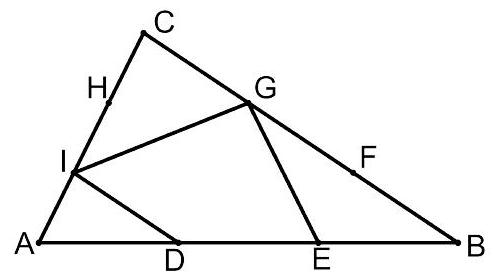
\includegraphics[max width=\textwidth, center]{2024_11_21_8c59a2d079965ff631b7g-1}

\section*{ZADANIE 2.}
Duża bombka na choinkę kosztuje 5 monet, średnia 3 monety, a za trzy małe bombki w kształcie aniołka trzeba zapłacić jedną monetę. Za sto monet kupiono sto bombek na choinkę. Ile wśród nich było dużych, średnich i małych bombek? Rozważ wszystkie możliwości.

\section*{ZADANIE 3.}
W zbiorze liczb rzeczywistych rozwiąż układ równań

\[
\left\{\begin{array}{l}
a b=a+b+1 \\
b c=b+c+2 \\
a c=a+c+5
\end{array}\right.
\]

\section*{ZADANIE 4.}
Znajdujemy ostateczną sumę cyfr liczby naturalnej - sumujemy jej cyfry i jeżeli wynik nie jest jednocyfrowy, to operację powtarzamy do skutku. Na przykład ostateczną sumą cyfr liczby 78987 jest 3 , gdyż \(7+8+9+8+7=39,3+9=12,1+2=3\) i do jej obliczenia potrzeba trzykrotnego sumowania cyfr. Podaj najmniejszą liczbę, która wymaga czterokrotnego sumowania, aby wyznaczyć ostateczną sumę jej cyfr.

\section*{ZADANIE 5.}
Bartek rzucił sto razy kostką do gry i zsumował liczby wyrzuconych oczek. Czy jest możliwe, aby suma ta była równa 211, jeżeli ani razu nie wypadła liczba parzysta?


\end{document}